\section{Introduction}

\begin{wrapfigure}{r}{0.6\textwidth}
    \centering
    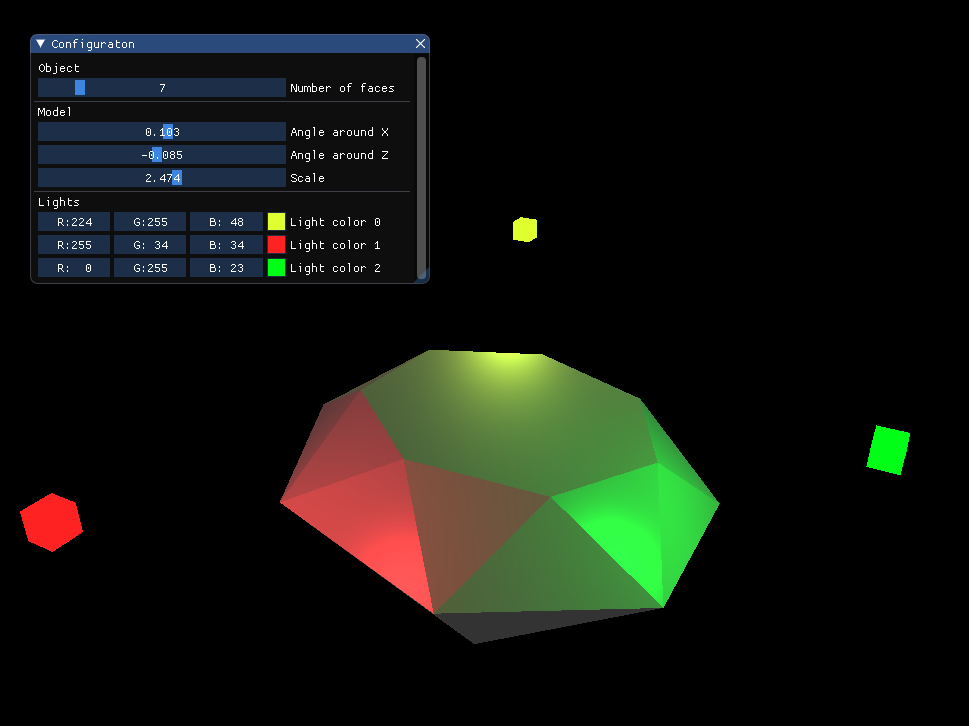
\includegraphics[width=0.59\textwidth]{screenshot_software}
\end{wrapfigure}

Pour ce projet d'IN55, nous avons choisi le sujet de \emph{génération
d'objets paramétriques}.

Dans le cadre de ce sujet, nous avons fait le choix de nous concentrer sur le paramétrage
et le rendu 3D d'un \emph{diamant}.
Dans un premier temps, le maillage du diamant et le système de lumière a été implémenté.
Il est possible de configurer le nombre de faces inférieures du diamant ainsi que
les lumières projetées sur le diamant qui est opaque.

Dans un second temps, nous avons essayé de modéliser les réflexions en rendant le diamant
transparent.

Ce rapport contient la notice d'utilisation du logiciel, en présente son architecture
et détaille les différentes méthodes que nous avons mises en place.
Le cœur de ce projet étant la génération paramétrique d'un diamant, cela concerne
donc principalement la création algorithmique d'un maillage 3D, mais une piste de
recherche pour faire des réflexions réalistes est aussi été présentée.

